\documentclass[a4paper, 10pt]{article}

\usepackage[utf8]{inputenc}
\usepackage[T1]{fontenc}
\usepackage{lmodern}
\usepackage[english]{babel}
\usepackage{graphicx}
\usepackage{hyperref}
\usepackage[margin=3cm]{geometry}
\usepackage[section]{placeins}
\usepackage[noend]{algpseudocode}
\usepackage{amssymb}
\usepackage{caption}
\usepackage{xcolor}


\newcommand{\GE}{TO-Multicast}
\newcommand{\PE}{Calvin}

\newboolean{showcomments}
\setboolean{showcomments}{true}
\ifthenelse{\boolean{showcomments}}
{ \newcommand{\mynote}[3]{
   \fbox{\bfseries\sffamily\scriptsize#1}
   {\small$\blacktriangleright$\textsf{\emph{\color{#3}{#2}}}$\blacktriangleleft$}}}
{ \newcommand{\mynote}[3]{}}

\newcommand{\Li}[1]{\mynote{Li}{#1}{blue}}
\newcommand{\Ch}[1]{\mynote{Ch}{#1}{green}}

% Custom definition
\algblockdefx[VARIABLES]{Variables}{EndVariables}
    {\textbf{Algorithm variables}}
    {}

\algblockdefx[UPON]{Upon}{EndUpon}
    [1]{\textbf{upon} #1}
    {}
\newcommand{\IndentState}{\State\hspace{\algorithmicindent}}
\algrenewcommand{\algorithmiccomment}[1]{\State\textit{{\footnotesize//} #1}}


\title{Adaptive ordering protocol for partially replicated state machine}
\author{Charles Vandevoorde}
\date{\today}

\begin{document}
\maketitle

\section{Purpose}

Skewness in distributed data store is a well-known problem and the topic is still an active area of research.
Most of the research are focused on partition skewness which is the difference of workload between
partitions in the system. Other data access pattern can also introduce a difference of workload which can
reduce the performance of the system. This protocol aims to reduce one of this type of skewness introduced by
partitioning, mainly multi-partition operations access pattern skewness. \Li{Tesdfasdfst}

As multi-partition operations (MPOs) are involving multiple partitions, we can assume that the data access pattern
between the different partitions will not be the same. A partition will certainly have more \textit{affinity}
for some partitions than others.

The protocol introduced here aims to reduce latency of MPOs dispatching and ordering for this kind of skewed workload.

\section{Challenges} \label{sec:challenges}
   The main difficulty in combining the use of {\GE} and {\PE} comes from the fact that each of them
   use different mechanisms to determine the order of transactions within each partition: {\GE}
   orders transactions by their timestamps; while {\PE} does not have the notion of timestamps, the
   use of synchronized rounds across all partitions allow a deterministic transactions ordering.
   % \Li{rephase, transactions within a round has to be further deterministically ordered}.
   Figure
   \ref{fig:inconsistency} exemplifies a case where two partitions can order transactions
   differently. In the figure, $P1$ tries to dispatch $T5$ to $P3$ and $P4$. $P2$ also tries to
   dispatch $T4$ to $P3$ and $P4$. Note that since $P1$/$P2$ both communicate with $P3$ and $P4$,
   $T4$/$T5$ will be dispatched to $P3$ and $P4$ with different `identifies'\Ch{What does identifies
   means in this context?}. However, if there is
   no mechanism to compare two transactions dispatched by {\GE} and {\PE}, $P3$ and $P4$ may execute
   $T1$ and $T2$ in different order.

   To mitigate this problem, we can associate transactions dispatched by \PE{} also with one
   timestamp. As such, a partition can order transactions simply by their timestamps, as in {\GE}.
   When a timestamp is assigned with \GE{}, every partition involved participates in the
   assignation; while \PE{} assigns the timestamp at the origin partition and requires ordering at the destination.
   Thus, \PE{} transactions are discovered each round by others partitions when \GE{} transactions are known in advance.
   \PE{} partitions must inform other partitions about their states every round to make sure, as
   \GE, that partitions are aware of pending transactions. Violating this condition can easily break the
   total order if partitions doesn't know which transactions' timestamp could be dispatched next.


   % Though, the transaction execution should b
   % Though, the assignment of timestamps to a batch of transactions should stick to the following two
   % conditions: 1) a batch of transactions should be assigned the same timestamp across all
   % partitions that communicate by {\PE}\Ch{Actually, transactions in a batch could have different
   % timestamps value (if there is \GE{} communication for example). A transaction must have the same
   % timestamp across all partitions but it looks like it's obvious to respect the total order.},
   % 2) in all partitions, the timestamp of a batch of
   % transactions should be smaller than the timestamp of any transaction that may be dispatched to
   % this partition later. Obviously, violating this condition can easily break the total order
   % guarantee \Li{rephase, define more clearly total order guarantee}.


\begin{figure}
    \centering
    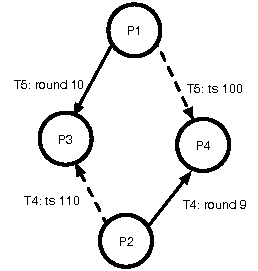
\includegraphics[width=0.5\textwidth]{assets/inconsistency}
    \caption{Example of partitions using different protocols}
    \label{fig:inconsistency}
\end{figure}


\section{Protocol}

\subsection{Description}\label{sec:protocol}

The basic idea of the protocol is to use two communication schemes with different characteristics to dispatch and order
MPOs. Those protocols are called Calvin and TO-MULTICAST. Calvin is a round-based ordering protocol, provides an optimal
latency but requires involvement from every node in the system with periodic communications. TO-MULTICAST is a genuine (involves only
partitions required by the transaction), based on logical clock but requires more communication steps.

A partition communicates with another partition with either Calvin or TO-MULTICAST. Calvin is used when
the two partitions talk a lot to each other. TO-MULTICAST is used when partitions are not communicating much together
to avoid the overhead of Calvin involvement in the ordering. A transaction can be dispatched and ordered with only the Calvin sequencer or
TO-MULTICAST or both depending on the partitions involved.

To totally order MPOs, a common source of truth between the two protocols needs to exist. Logical clock
is used as a single source of truth, even with Calvin ordered only MPOs. We will see how during the protocol breakdown.

The protocol can be decomposed in different steps:

\begin{description}
    \item[Init phase (line \ref{alg:line:init}-\ref{alg:line:init:end})] First, we get a batch containing MPOs collected in
        a small timeframe. Next, protocols needed to dispatch an MPO are saved inside the transaction as a metadata.
        This metadata ensures a consistent dispatching even when a switching occurs during the dispatching and ordering
        of the transaction.

    \item[Replication phase (line \ref{alg:line:replication}-\ref{alg:line:replication:end})]
        For fault tolerance, MPOs are replicated across nodes inside the same
        partition. An intra-partition concensus is also made on the Local
        Maximal Executable Clock (LMEC) by taking the minimum of all proposed
        LMEC inside the partition. The LMEC guarantees that no transaction with a
        smaller logical clock than the LMEC will be dispatched with \PE{} from this partition.
        This guarantee means that another partition can safely execute transactions
        with a smaller timestamp than the LMEC and still respect the ordering between those
        two partitions. As explained in section \ref{sec:challenges}, the LMEC will inform
        the state of the partition to other partitions.

    \item[Genuine dispatching (line \ref{alg:line:genuine_dispatch}-\ref{alg:line:genuine_dispatch:end})]
        When a transaction in the batch has to be dispatched to some partitions using \GE, the transaction will be dispatched
        to those partitions with TO-MULTICAST. The protocol keeps track of the transactions dispatched by genuine
        by adding them to a special queue
        called $pendingQ$. The dispatching is done completely asynchronously and the main loop
        doesn't wait for the transaction to be decided by the genuine protocol.

    \item[Clock assignation phase (line \ref{alg:line:clock_assign_genuine} and \ref{alg:line:clock_assign_calvin}-\ref{alg:line:clock_assign_calvin:end})]
        Each round, the protocol check if the genuine implementation has transactions which are decided (dispatched and
        in order). Those transactions are assigned a logical clock by the TO-MULTICAST protocol
        where each logical clock is consistent across partitions.

        TO-MULTICAST assigns logical clock in a propose-decide fashion. First, every node sends its maximal logical clock
        to the other nodes involved. Next, each node decides the logical clock by taking the maximal value and updates
        its logical clock to the maximal clock received.
        Finally, a transaction is decided by TO-MULTICAST when the transaction has the smallest logical clock
        compared to every transaction which are still being ordered. This ensures that decided transactions respect the total
        order. %\Ch{May be not clear but this is specific to TO-MULTICAST. It's not very important.}.

        When the clock is assigned, the transaction can be in two different states depending if it still needs
        dispatching with the Calvin sequencer or not:
        \begin{description}
            \item[READY state] means that the transaction needs to be dispatched with the Calvin sequencer.
            \item[EXECUTABLE state] means that the transaction is waiting to be executed.
        \end{description}

        When a transaction in the batch doesn't require any genuine dispatching, the transaction is assigned a
        special clock value $calvin\_logical\_clock$ which was defined during the previous round
        \Li{big question: do we need to assign these transactions timestamp? Isn't it enough to just
        execute them in front of all transactions in that batch?}\Ch{No because \GE{} transactions
        executions are not bounded on a round which means that some partitions may already have executed some
        transactions in round $X_i$ while other partitions will execute them in round $X_{i+\lambda}$}.
        The detail will be explained
        later. As the transaction still requires Calvin sequencing, the transaction is in \textbf{READY} state.

    \item[Calvin sequencer dispatching phase (line \ref{alg:line:calvin_dispatch}-\ref{alg:line:calvin_dispatch:end})]
        As required by the Calvin sequencer protocol, a message will be
        send to every Calvin connected partition. This message will include two informations:
        \begin{itemize}
            \item Transactions with a \textbf{READY} state in this round
            \item The local MEC calculated during this round
        \end{itemize}

        Next, the protocol waits for messages coming from the other Calvin sequencer connected partitions.
        When every message is received, we have a list containing transactions and every local MEC sent.
        Transactions received can directly added to the execution queue.

    \item[Execution phase (line \ref{alg:line:execution}-\ref{alg:line:execution:end})]
        Before the execution, the global MEC (Maximal Executable Clock) needs to
        be calculated by taking the minimum LMEC received (see
        \textit{Replication phase} and \textit{Calvin sequencer dispatching phase}). The MEC provides a
        bounded clock execution for a round to ensure synchronization between sub-protocols (genuine and Calvin sequencer).
        This limitation ensures that a partition $P_a$ doesn't
        execute a transaction $T_x$ with a clock value of $C_{T_x}$ when a partition $P_b$ has a
        transaction $T_y$ which has not yet been dispatched with the Calvin sequencer with a
        possible future logical clock $C_{T_y}$ such as $C_{T_x} > C_{T_y}$.

        With the MEC calculated, we can execute transactions which have a logical clock lower than the MEC.

    \item[Calvin sequencer value update (line \ref{alg:line:val_update}-\ref{alg:line:val_update:end})]
        Before starting a new round, important variables need be updated
        to ensure correctness in the following rounds.

        First, the $calvin\_logical\_clock$ is the logical clock value given to transactions which aren't assigned a
        logical clock by the genuine protocol (i.e. Calvin only transactions). One condition is
        required to ensure total order property: $calvin\_logical\_clock$ value should have a
        greater timestamp than any executed transactions during the round. This condition is
        required to make sure that transactions will be executable in the following rounds.
        As the MEC is bounding the execution, each \PE{} connected partition knows the
        maximal clock executed. For simplicity, the $calvin\_logical\_clock$ is the maximum of
        all LMEC received which is always greater than the maximal clock executed.

        Second, the logical clock of the genuine protocol is updated only to make sure that our protocol advances when
        no genuine communication occurs. As explained in the \textit{Clock assignation phase}, the logical clock
        is updated by the genuine protocol itself but when no genuine communication happens, the logical clock is not updated.
        As explained in the \textit{Replication phase}, the LMEC is based on the logical clock of the genuine protocol.
        If this logical clock is not updated, we may no longer execute transactions as the MEC will not increase.

\end{description}

\subsection{Pseudocode}

\begin{algorithmic}[1]
    \small
    \Variables
        % \State $opQ$: queue containing MPO in different states.
            % \IndentState \textbf{PENDING}: waiting genuine dispatching
            % \IndentState \textbf{READY}: waiting low latency dispatching
            % \IndentState \textbf{EXECUTABLE}: waiting execution
        \State $pendingQ$: a queue storing MPO waiting genuine dispatching
        \State $executablePQ$: a priority queue storing MPO waiting to be executed
        \State $genuine$: genuine sub-protocol implementation
        \State $round$: round number
        \State $low\_latency\_clock$: clock value assigned to exclusive low latency MPO
        \State $genuine$: interface to the genuine protocol
    \EndVariables

    \Upon{new round}
        \State $MPOs\gets$ get batched MPOs \label{alg:line:init}
        \For{$MPO \in MPOs$}
            \For{$p \in MPO.partitions()$}
                \State $MPO.protocols[p]\gets get\_protocol(p)$
            \EndFor
        \EndFor \label{alg:line:init:end}
        \State $local\_mec\gets get\_mec(genuine, decided\_by\_genuine)$
        % \Comment{Intra-partition consensus}
        \State
        \State C-PROPOSE([$MPOs$, $local\_mec$]) \label{alg:line:replication}
        \State \textbf{wait} C-DECIDE([$MPOs$, $local\_mec$]) \label{alg:line:replication:end}
        \State
        \Comment{Store transactions which need Calvin sequencing.}
        \State $readyQ \gets$ new queue()
        \For{$MPO \in MPOs$}
            \If{$\textbf{GENUINE} \notin MPO.protocols()$}
                \State $MPO.setLogicalClock(calvin\_logical\_clock)$ \label{alg:line:clock_assign_calvin}
                \State $readyQ.add(MPO)$ \label{alg:line:clock_assign_calvin:end}
            \Else
                \State $genuine.Send(MPO)$\label{alg:line:genuine_dispatch}
                \State $pendingQ.add(MPO)$\label{alg:line:genuine_dispatch:end}
            \EndIf
        \EndFor
        % \Comment{Classify decided genuine MPO}
        \State
        \State $decided\_by\_genuine\gets genuine.get\_decided()$ \label{alg:line:clock_assign_genuine}
        \For{$MPO \in decided\_by\_genuine$}
            % \If{$MPO \in opQ.withState(\textbf{PENDING})\ \&\&\ \textbf{LOW\_LATENCY} \in MPO.protocols()$}
            \If{$MPO \in pendingQ\ \&\&\ \textbf{LOW\_LATENCY} \in MPO.protocols()$}
                % \State $opQ.changeState(MPO, \textbf{READY})$
                \State $pendingQ.remove(MPO)$
                \State $readyQ.add(MPO)$
            \Else
                % \State $opQ.changeStateOrAdd(MPO, \textbf{EXECUTABLE})$
                \State $executablePQ.add(MPO)$
            \EndIf
        \EndFor \label{alg:line:get_multicast:end}
        % \Comment{Dispatch with low latency protocol}
        \State
        \State {Send the local\_mec and readyQ MPOs for every low latency communicating partition} \label{alg:line:calvin_dispatch}
        % \State Send low latency message to every low latency protocol connected partition.
            % \textit{For partition $P$, we send MPOs involved with $P$ and $local\_mec$}.
        % \State $opQ.changeStates()$
        \State $executablePQ \gets executablePQ + readyQ$
        % \State $opQ.clearState(\textbf{READY})$
        \State $received\_MPOs, mecs \gets$ \textbf{wait} messages from low latency protocol connected nodes \label{alg:line:calvin_dispatch:end}
        \State
        \State $mec \gets min(mecs)$ \label{alg:line:execution}
        % \Comment{Execute MPOs}
        \State
        % \For{$MPO \in sort(opQ.withState(\textbf{EXECUTABLE}))$}
        \For{$MPO \in executablePQ$}
            \If{$MPO.logical\_clock < mec$}
                \State Execute $MPO$
                % \State $opQ.remove(MPO)$
                \State $executablePQ.remove(MPO)$
            \Else
                \State \textbf{break}
            \EndIf
        \EndFor \label{alg:line:execution:end}
        \State
        \State $calvin\_logical\_clock \gets max(mecs)$ \label{alg:line:val_update}
        \State $genuine.logical\_clock \gets max(genuine.logical\_clock, calvin\_logical\_clock)$ \label{alg:line:val_update:end}
        \State
        \State $round \gets round+1$

    \EndUpon
\end{algorithmic}

\subsection{Example}

\begin{figure}
    \centering
    \includegraphics[width=0.5\textwidth]{assets/partition-organization}
    \caption{Example of partitions using different protocols}
    \label{fig:partition}
\end{figure}
\begin{figure}
    \centering
    \includegraphics[width=1.2\textwidth]{assets/timing-mec}
    \caption{Timing diagram representing the ordering of two transactions \textbf{A} and \textbf{B}.\\
    \textit{Horizontal arrows represent the time and black point on them informs a round change.
    Dashed vertical line represents a genuine agreement on the logical clock and normal vertical line are
    Calvin sequencer messages.}}
    \label{fig:timing}
\end{figure}

As the protocol explanation can be a bit abstract, here is an example which contains four partitions and two transactions
to order. Figure \ref{fig:partition} represents the protocols used to communicate between the partitions. As described
in the schema, only partition 1 and 2 are talking together with the Calvin sequencer. Every other partition pair is communicating
with the genuine protocol. For more clarity, we are only assuming one node per partition.

The two transactions will be received approximately at the same time at the partition 1 and 3. The partition 1 receives the
transaction \textbf{A} which also requires dispatching on partition 0 and 2. The partition 3 receives the transaction \textbf{B} which
also requires dispatching on partition 2. The ordering of those two partitions is schematized in Figure \ref{fig:timing}.
In the following paragraphs, each transaction dispatching will first analyzed separatly and afterwards, the ordering relation
and the execution will be discussed.

\paragraph{Transaction A.} As this transaction has a genuine and a Calvin connected partition, the protocol first needs to dispatch
    the transaction with the genuine protocol to assign it a logical clock. After some time, partition 0 and 1 agree on a logical clock
    of 213. Next, the transaction will dispatched with the Calvin sequencer at the round 18 as the round 17 had already begun when
    transaction \textbf{A} was decided. At round 18, partitions 0, 1 and 2 have the transaction \textbf{A} in their execution queue.
    The actual execution will be discussed in the last paragraph.

\paragraph{Transaction B.} This transaction only requires a genuine dispatching which provides, at the end, a logical clock
    of 247. At round 17, the transaction \textbf{B} is in the execution queue of partition 2 and 3.

\paragraph{The execution of A and B.} As shown in Figure \ref{fig:timing}, the transaction \textbf{B} is available (round 17)
    before \textbf{A} (round 18) even if \textbf{A} has a smaller logical clock. To ensure that transaction \textbf{B} is
    not executed before \textbf{A}, \textbf{B} needs to be delayed until at least transaction \textbf{A}'s execution to avoid breaking
    the total order.

    The MEC is providing this delay by bounding the logical clock execution for every round. As you can see,
    for round 17, $MEC=min(250, 201)=201$ and as $201 < (B_{clock} = 247)$,
    the transaction \textbf{B} can't be executed in round 17. In round 18, as transaction \textbf{A} has been decided
    by the genuine protocol and dispatched by the Calvin sequencer,
    the partition $1_{LMEC} > 213$ and we have the relation $(A_{clock} = 213) < (B_{clock} = 247) < MEC$
    which means that \textbf{A} and \textbf{B} can be executed in total order in this round.

\subsection{Correctness proof}
We are assuming two transactions $T_a$ and $T_b$. $T_a \prec T_b$ relation implies $T_a$ is ordered before
$T_b$ on every correct process involved in $T_a$ and $T_b$. The "$\prec$" relation is the total ordering property.
$T_a < T_b$ for a process $P_a$ implies that $T_a$ is ordered before $T_b$ inside process $P_a$ and
has no other garantee on the ordering for other processes. The "$<$" relation is the local ordering property. \\

Assume our sequencer receives two multi-partition transactions $T_x$ and $T_y$ on two different partitions.
Assume $T_x$ and $T_y$ are accessing two common partitions $P_a$ and $P_b$. By their timestamp
values $t_{T_{x}}$ and $t_{T_x}$, the total order relation is expected to be $T_x \prec T_y$.
By contradiction, we assume that we have $T_x < T_y$ on partition $P_a$ and $T_y < T_x$ on partition
$P_b$ which break the total order property. A violation of total order could happen because:
\textbf{a.} $t_{T_{a,b}}$ has a different timestamp value between partition $P_a$ and $P_b$. \textbf{b.}
If $T_x$ and $T_y$ have a consistent timestamp across partitions, partition $P_b$ executes $T_y$
before $T_x$ because $P_b$ doesn't know that a transaction $T_x$ exists such as $T_x \prec T_y$.

% Given an expected total order relation such as $T_x \prec T_y$ and $T_x$ is not yet received by
% partition $P_b$, $P_b$ executes $T_y$ before $T_x$
% \Li{I do not understand why b is the only possible case after excluding a. Shouldn't you also mention b in this case?}.

A transaction can be dispatched to its involved partitions either only using
one of the communication patterns, or using a combination of both, which we
call a \textit{hybrid} dispatching. In the following text, we analyze whether
the above cases are possible per dispatching type.

First, we examine if case \textbf{a.} is possible for each dispatching type for a transaction $T_x$
involving multiple partitions:

\begin{description}
    \item[Genuine dispatching] TO-MULTICAST properties\footnote{\url{ftp://ftp.irisa.fr/techreports/1998/PI-1162.ps.gz}}
        ensures a consistent logical clock across nodes involved in the transaction.

        When TO-MULTICAST assigns a logical clock to a transaction, the protocol is executed in three steps:
        \begin{enumerate}
            \item Each partition makes an intra-partition consensus to agree on a vote
                for the final logical clock value.
            \item Every node sends its logical clock vote to the other nodes involved in the transaction.
            \item Each node uses the maximal vote received to be final logical clock
                for the given transaction.
        \end{enumerate}
        As every node choose the maximal vote received, it's evident that every node will have the
        same logical clock.

    \item[Calvin sequencing] Before $T_x$ is dispatched, the partition receiving the transaction $T_x$ will assign
        a logical clock which is equals to $calvin\_logical\_clock$. As the $calvin\_logical\_clock$ is
        based on the LMEC which is the result of intra-partition consensus, the $calvin\_logical\_clock$ will
        be consistent between replicas inside a transaction. The inter-partition logical clock value will also stay
        consistent as the logical clock is decided only by one partition.

    \item[Hybrid dispatching] $T_x$ is dispatched in two steps. First, $T_x$ is dispatched with
        the genuine protocol to partitions which are communicating with the genuine protocol.
        When $T_x$ is decided by the genuine protocol, it has a logical clock which is consistent as seen above
        across the genuine partitions. Second, $T_x$ is dispatched with the Calvin sequencer with the same logical
        clock. Every involved node in $T_x$ now has received the transaction with a consistent logical clock.
\end{description}

Next, we examine whether case \textbf{b.} is possible for each dispatching type with two multi-partitions
transactions $T_x$ and $T_y$ with a common partition $P_a$.

\begin{description}
    \item[Genuine dispatching] TO-MULTICAST properties ensure that the transaction $T_x$ will be decided
        iff there is no transaction $T_y$ such as $T_y \prec T_x$ relation is possible. If there is no
        transaction with a smaller logical clock, no transaction will ever have a smaller
        logical clock and thus, no transaction will ever break the total order.

    \item[Calvin sequencing] Unlike the base Calvin sequencer, transactions are not simply deterministically
        ordered and then executed. Transactions are assigned a logical clock to make sure the ordering is
        consistent with other transactions. The logical assigned to a Calvin sequencer only transaction $T_x$
        has the value of $calvin\_logical\_clock$ which was calculated during the previous round. This value was
        calculated by taking the maximum of all LMEC received such as $calvin\_logical\_clock_{r}=max(LMECs)$.
        As $MEC_{r-1} = min(LMECS)$ and $MEC_{r-1}$ is the maximal logical clock executed during the previous round,
        the transaction $T_x$ can be ordered safely.

        Even if some transactions have the same logical clock, transactions can be deterministically
        ordered just like the Calvin sequencer do.

    \item[Hybrid dispatching] Since an hybrid transaction $T_x$ delays its Calvin sequencing to get a
        logical clock with the genuine dispatching, the protocol must ensure that execution of $T_x$
        respects the total order. The total order is consistent if no transaction with a smaller logical clock
        than transaction $T_x$ is received in the future when $T_x$ is executed.
        The execution guard is given by the MEC which limits the execution
        to transactions which only have a smaller logical clock than the MEC value.

        MEC only apply to partitions communicating with the Calvin sequencer because TO-MULTICAST already ensures
        total order by only deciding a transaction when it has the smallest logical clock. For partitions talking with the Calvin
        sequencer, the MEC is an agreement of the maximal executable clock of every partition and every replica
        (thanks to the consensus on the LMEC). As every partition sends the maximal executable clock locally and
        the MEC is the minimum of those values, no node can execute a transaction which breaks the total order.
\end{description}

\section{Protocol switching}

The protocol switching is divided in different parts. First, a different protocol is used between
TO\_MULTICAST $\rightarrow$ Calvin sequencer and Calvin sequencer $\rightarrow$ TO\_MULTICAST.
In addition, when we are switching from TO\_MULTICAST to the Calvin sequencer, we need to handle different
cases because those cases are more tricky as we will see later.

For the sake of simplicity, the protocol switching will be described as a state machine which
breaks the switching into different steps. The switching is executed after each dispatching round without
blocking it.

\subsection{Common}

The first step of a switching is an agreement between the two partitions. This agreement will make sure that
every node in both partitions are aware of the switch. If one of the partition is already busy with an other
switch, the switch initialization is aborted and the switch will be retried later on.
% \Li{Why can't this request be queued? In the current manner, is it possible that some switching may never be triggered (no progress)?}.
The agreement is also used to agree on several values that will be useful in the switch and saved in an object called $switch\_metadata$ for
convenience:

\begin{description}
   \item[$switching\_round$] is a round value at which both partitions can switch in a synchronized fashion
   \item[$partition\_type$] is the type of the other partition that will be used to decide which switching protocol should be used
\end{description}

As explained above, the switch is divided in different cases depending on the type of protocol currently used.
Line \ref{alg:line:init_switch} to \ref{alg:line:init_switch:end} handles the different cases possible.
Line \ref{alg:line:init_switch_genuine} to \ref{alg:line:init_switch_genuine:end} handles the different cases when
switching from TO\_MULTICAST to the Calvin sequencer depending on the partition type. A partition can have
one of those three types:

\begin{description}
    \item[Full low latency] is a partition which communicates only with the Calvin sequencer.
    \item[Full genuine] is a partition which communicates only with TO-MULTICAST.
    \item[Hybrid] is a partition which communicates with TO-MULTICAST to some partitions and
        with Calvin to the others.
\end{description}

Each case is then explained separately for more clarity as they are completely isolated from each other.

\subsubsection{Pseudocode}

\begin{algorithmic}[1]
    \Variables
        \State $state$: current state of the switching
        \State $switch\_metadata$: metadata based on the agreement of the two switching partitions
    \EndVariables

    \Upon{switching agreement with partition $P_{switch}$}
        \If{$get\_protocol(P_{switch}) = LOW\_LATENCY$} \label{alg:line:init_switch}
            \State $state \gets INIT\_SWITCH\_TO\_GENUINE$
        \Else
            \If{$switch\_metadata.partition\_type = FULL\_GENUINE$ \textbf{or} \par\hspace{2cm} $get\_this\_partition\_type() = FULL\_GENUINE$} \label{alg:line:init_switch_genuine}
                \State $state \gets INIT\_SWITCH\_TO\_LOW\_LATENCY\_FULL\_GENUINE$
            \Else
                \State $state \gets INIT\_SWITCH\_TO\_LOW\_LATENCY\_HYBRID$
            \EndIf \label{alg:line:init_switch_genuine:end}
        \EndIf \label{alg:line:init_switch:end}
    \EndUpon
\end{algorithmic}

\subsection{Calvin sequencer $\rightarrow$ TO-MULTICAST} \label{sec:calvin-to-genuine}

Switching from the Calvin sequencer to TO-MULTICAST requires 4 steps:

\begin{description}
    \item[Transition phase (line \ref{alg:line:gen:transition}-\ref{alg:line:gen:transition:end})]
        When the switching round happens (agreed upon during the \textit{init} phase), both partitions
        will change from Calvin sequencer protocol to a transition protocol. This transition protocol is
        running both protocol at the same time meaning that new transactions received will be dispatched
        with the genuine protocol for the switching partitions while the Calvin sequencing message will still be sent \Li{why do we need to have both protocols running together? Isn't it enough to keep delivering message using Calvin until the switch round has reached?} to ensure the next step in the switching will eventually terminate.

    \item[Waiting for required Calvin sequencing (line \ref{alg:line:gen:round})]
        Before switching to the genuine protocol, the switching protocol
        needs to make sure that transaction no longer requires Calvin sequencing with the switching partition \Li{when can we know this condition? And can't this round be known in advance in the previous phase?} by checking the pending transactions queue.
        Otherwise, some transactions may not be dispatched to the switching partition which will break
        the total order property. It means that the next step in the protocol switch is delayed until this condition is
        fulfilled.

    \item[Switching round agreement (line \ref{alg:line:gen:round} to \ref{alg:line:gen:round:end})]
        Like the \textit{init} phase, an agreement is made between both switching partition and their respective replicas
        to find a round to switch. This agreement takes the form of a consensus with two primitives $A-PROPOSE$ and $A-DECIDE$.

    \item[Genuine switch (line \ref{alg:line:gen:switch} to \ref{alg:line:gen:switch:end})]
        When the switching round is reached, the partition can switch to the genuine partition.
\end{description}

\subsubsection{Pseudocode}
\Li{For the pseudo-code: when is switching round decided?}\Ch{The first switching round is decided during the common phase}

\begin{algorithmic}[1]
    \Upon{$state = INIT\_SWITCH\_TO\_GENUINE$ \textbf{and} \par\hspace{0.8cm}$current\_round = switch\_metadata.switching\_round$}\label{alg:line:gen:transition}
        \State $state \gets FINISH\_LOW\_LATENCY\_DISPATCHING$
        \State $set\_protocol(P_{switch}, TRANSITION)$
    \EndUpon\label{alg:line:gen:transition:end}

    \Upon{$state = FINISH\_LOW\_LATENCY\_DISPATCHING$ \textbf{and}\par\hspace{0.8cm} no transaction left for Calvin dispatching with partition $P_{switch}$}\label{alg:line:gen:round}
        \State $A-PROPOSE(P_{switch}, current\_round + delta)$
        \State $switch\_metadata.switching\_round \gets wait\ A-DECIDE(P_{switch})$
        \State $state \gets SWITCH\_TO\_GENUINE$
    \EndUpon\label{alg:line:gen:round:end}

     \Upon{$state = SWITCH\_TO\_GENUINE$ \textbf{and}\par\hspace{0.8cm} $current\_round = switch\_metadata.switching\_round$}\label{alg:line:gen:switch}
        \State $set\_protocol(P_{switch}, GENUINE)$
        \State $state \gets$ \textbf{null}
     \EndUpon\label{alg:line:gen:switch:end}
\end{algorithmic}

\subsection{TO-MULTICAST $\rightarrow$ Calvin sequencer {\tiny$\blacksquare$} One or two full genuine}\label{sec:genuine-to-calvin-full-genuine}

Before switching to the Calvin sequencer, both partitions need to have the same round number. Otherwise,
the periodic message sent by the partitions won't be synchronized and the two switching partitions will block.

If at least one of the switching partition is a full genuine partition, the switching is really straightforward because
round number of full genuine partitions can be changed without interfering with the protocol as no Calvin sequencing
message needs to be sent.

The protocol can be described in two steps:

\begin{description}
    \item[Round change (line \ref{alg:line:calvin_1:round}-\ref{alg:line:calvin_1:round:end})]
        As explained above, the round number needs to be synchronized between the switching partitions.
        The round update depends on the type of the partitions involved:

        \begin{description}
            \item[Two full genuine partitions] \sloppypar{In the \textit{init} phase, both partitions made an agreement on
                some values such as $switch\_metadata.switching\_round$. As we are creating two new hybrid partitions,
                any round value is valid as long as it's synchronized. $switch\_metadata.switching\_round$ is used because
                it's already available and the value is same on every node in the switching partitions.}

            \item[One hybrid and one full genuine partitions] An hybrid partition is talking with other partitions with
                the Calvin sequencer protocol which means it's impossible to change the round number without also switching
                those connected partitions. Fortunately, the full genuine partition can switch to any round number.
                The full genuine partition will wait for the first Calvin sequencing message from the hybrid
                partition to receive the current round value.
        \end{description}

        After updating round number, switching partitions switch their protocol to the transition
        protocol (like \textit{Calvin sequencer $\rightarrow$ TO-MULTICAST}).
    \item[Calvin sequencer switch (line \ref{alg:line:calvin_1:switch}-\ref{alg:line:calvin_1:switch:end})]
        Before switching to the Calvin sequencer protocol, a round is executed with the transition protocol
        to synchronize LMEC between the switching partitions. LMEC are required to make sure that variables
        such as $calvin\_logical\_clock$ are updated before receiving transactions with the Calvin sequencer.
        \Li{why? Can't we use each partition's existing LMEC?}
        \Ch{No because the LMEC from the switching partition is not yet received because the communication was using
           genuine before so no LMEC send.}
        After this synchronization round, the protocol can be updated to the Calvin sequencer.
\end{description}

\subsubsection{Pseudocode}

\begin{algorithmic}[1]
    \Upon{$state = INIT\_SWITCH\_TO\_LOW\_LATENCY\_FULL\_GENUINE$} \label{alg:line:calvin_1:round}
        \If{$get\_partition\_type() = FULL\_GENUINE$ \textbf{and}\par\hspace{1.2cm} $other\_partition\_type = FULL\_GENUINE$}
            \State $current\_round \gets switch\_metadata.switching\_round$
        \ElsIf{$get\_partition\_type() = FULL\_GENUINE$}
            \State $msg \gets$ wait LOW LATENCY message
            \State $current\_round \gets msg.round$
        \EndIf
        \State $switching\_round = current\_round$

        \State $set\_protocol(P_{switch}, TRANSITION)$
        \State $state \gets SYNCHRONIZE\_MEC$
    \EndUpon \label{alg:line:calvin_1:round:end}

    \Upon{$state = SYNCHRONIZE\_MEC$ \textbf{and} $current\_round = switching\_round + 1$} \label{alg:line:calvin_1:switch}
        \State $set\_protocol(P_{switch}, LOW\_LATENCY)$
        \State $state \gets$ \textbf{null} \label{alg:line:calvin_1:switch:end}
    \EndUpon
\end{algorithmic}

\subsection{TO-MULTICAST $\rightarrow$ Calvin sequencer {\tiny$\blacksquare$} Two hybrid}

As explained above, the Calvin sequencer requires connected partitions to have the same round number to
terminate a round. Every partition which is connected by Calvin and has the same round number at one time
compared to other partitions are forming a graph, called Calvin sequencer connected graph.

When we have two hybrid partitions, we can have two partitions which are in the same graph or in two
different graphs. When we are initializing the protocol switching, it is impossible to tell if
two partitions are in the same graph or not due to the network being asynchronous.

% Removed because consensus is now more clairly explained where it's used in the steps.
% Each time a message is send from a partition to another \Li{what kind of message?}, the communication must be a consensus to ensure
% consistency even in case of failure.

The protocol switching for two hybrid partitions requires updating the round number in one or two graphs
which can described in multiple steps:

\begin{description}
    \item[Graphs locking] Before updating the round number of the graphs, the protocol switch needs to make
        sure that no other switch occurs in the graph. This locking is required to, first, keep track of
        every partition involved in the graph and,
        % \Li{what do you mean 'make a map'? Do you mean just keeping track of the partitions?}
        second, avoid switching with other partition inside the graph
        to avoid unknown partition in the mapping. If there is already a switching occurring in the graph,
        the switch needs to be aborted and every partition locked should be unlocked.

        The graph locking can be implemented in different ways. We choose an implementation where the switching
        partitions are doing the heavy lifting which is easier to manage and reason about.
        The switching partition will run a consensus with every of its neighbours partitions to lock them. Every neighbour will share their
        own neighbours. Next, the switching partition will lock those partitions and receive neighbours information until
        every partition in the graph as been discovered.

        During the graph locking, the switching protocol can also discover that there is only one graph because both
        partitions are in the same graph.

   \item[Switching round agreement] If we use the same technique as \ref{sec:calvin-to-genuine} with $switching\_round$
       and we have two distinc graphs, we may block a graph for a non-negligeable amount of time because the two graphs have different
       round values. The lowest round value graph would have to catch up to the highest round value graph where the round difference could be
       big. The highest round value graph will need to wait and will block during the catch-up.

       To avoid blocking one graph, the two switching partition will agree on two different values. First, $switching\_round$
       will be the round value at which the graph will switch. This value is either the same if the protocol detects that we only
       had one graph or different if we have two distinc graphs. If we two different switching round value, we can reduce the
       blocking time but the two graphs will be at different round value. The same round value is given by $final\_round$ which
       jump the round value of both graphs to the same value. $final\_round$ is an agreement between the two switching partitions
       ensuring both graphs have the same round at the end.

    \item[Graphs round update propagation] Thanks to the round locking, the two switching
        partitions know which partitions are in their graphs. The
        round update propagation will be handled by the switching partitions. $switching\_round$ and $final\_round$ will
        be sent to every locked partition.
        % be sent in every round update message \Li{You mean the round propagation message will be sent to all other switching partitions?}.

    \item[LMEC Synchronization] Like in section \ref{sec:genuine-to-calvin-full-genuine}, before switching to the Calvin sequencer
        protocol, we need to switch to the transition protocol between the two switching partitions
        \Li{Just the two partitions, or also all connected partitions?}\Ch{Just the two switching partitions because other partitions are already sharing their LMEC
        because they are talking with Calvin.}
        after upgrading the round number. The transition protocol will synchronize the various values of the \textit{CaMu} protocol.
        \Li{Overall, can't LMECs be synchronized together during switching round agreement phase?}\Ch{No because to send Calvin message we need to have
           synchronized round number.}

    \item[Calvin sequencer switching] After one synchronization round, both switching partitions can switch to the Calvin
        sequencer protocol safely.
\end{description}

\subsubsection{Pseudocode}

For the sake of brevity, the protocol shown below is only described for the switching partition and not for partitions
involved in the graph.
\Li{replace launch graph locking with a few lines of brief brief description would be more clear}
\Ch{added a small pseudo-code to reflect what the algo is really doing.}

\begin{algorithmic}[1]
    \Variables
        \State $locked\_partitions$: a set containing partition ids of locked partition
    \EndVariables

    \Upon{$state = INIT\_SWITCH\_TO\_LOW\_LATENCY\_HYBRID$}
        % \State $launch\_graph\_locking()$
    \State $unvisited\_partitions \gets $ \textit{set(get every neighbour partition using \PE{})}
       \While{$unvisited\_partitions.size() != 0$}
           \State $partition\_id \gets unvisited\_partitions.pop()$
           \State $A-PROPOSE(partition\_id, PARTITION\_LOCK)$
           \State $unvisited\_partitions.add(wait\ A-DECIDE(partition\_id))$
           \State $locked\_partitions.add(partition\_id)$
       \EndWhile
    \EndUpon

    \Upon{\textit{locking is finished}}
        \State $A-PROPOSE(P_{switch}, (switching\_round, final\_round))$
        \State $(switching\_round, final\_round) \gets wait\ A-DECIDE(P_{switch})$
        \State $propagate\_round\_info(switching\_round, final\_round)$
    \EndUpon

    \Upon{$current\_round = switching\_round$}
        \State $current\_round \gets final\_round$
        \State $set\_protocol(P_{switch}, transition)$
        \State $state \gets SYNCHRONIZE\_MEC$
    \EndUpon

    \Upon{$state = SYNCHRONIZE\_MEC$ \textbf{and} $current\_round = final\_round + 1$}
        \State $set\_protocol(P_{switch}, LOW\_LATENCY)$
        \State $state \gets$ \textbf{null} \label{alg:line:calvin_1:switch:end}
    \EndUpon
\end{algorithmic}

\end{document}
